\section{Enunciado}
En este trabajo se procederá al análisis de tres circuitos:

\begin{itemize}
    \item Amplificador VFA - VFA.
    \item Amplificador VFA - CFA.
    \item Amplificador VFA - CFA, con red de compensación.
\end{itemize}

En cada circuíto, se harán análisis teóricos y simulaciones.

\subsection{Circuíto Propuesto}
En la siguiente figura se muestra un amplificador compuesto que deberá ser diseñado para obtener una ganancia global Avf = 20[dB], compensándolo para obtener una máxima planicidad de módulo ($M\phi = 65^o$).

    \begin{figure}[ht]
    	\centering
    	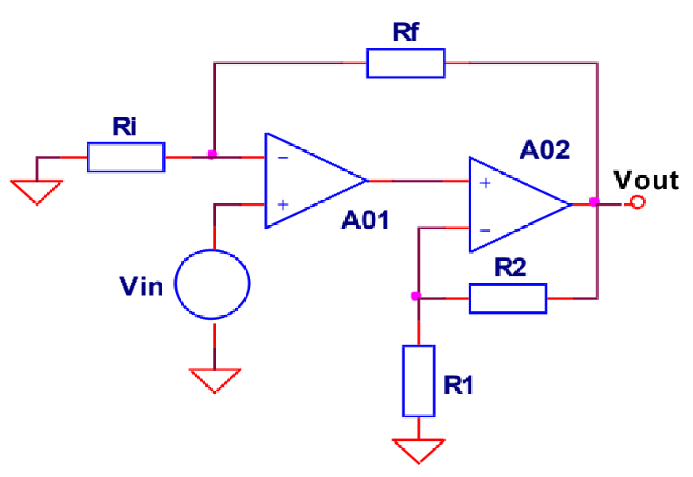
\includegraphics[height=5cm]{Imágenes/Circuito1.png}
    	\caption{Circuíto a analizar}
    \end{figure}

\subsubsection{VFA-VFA:}
 Utilizando las tecnologías VFA + VFA. como amplificador VFA se utilizará un \textbf{LM324} de dos polos ($Ad0 = 100 [dB], f_T = 1 [MHz], f_1 = 10[Hz], f_2 = 5.06 [MHz]$).\\
 
 \begin{itemize}
     \item Diseñar el amplificador compuesto VFA - VFA.
     \item Calcular el ancho de banda potencial, la frecuencia del polo de la función de transferencia a lazo cerrado y el ancho de banda a -3 [dB].
     \item Medir el ancho de banda a -3 [dB].
     \item Estimar el margen de fase obtenido en base a la respuesta al escalón del amplificador compuesto.
 \end{itemize}


\subsubsection{VFA-CFA:}
 Utilizando las tecnologías VFA + CFA. Se sugiere como amplificador VFA un \textbf{LM324} de dos polos ($Ad0 = 100 [dB], f_T = 1 [MHz], f_1 = 10[Hz], f_2 = 5.06 [MHz]$) y como CFA un \textbf{LM6181} con ($R_T= 2.37 [M\Omega], C_T = 4.8 [pF]$), cuya transimpedancia $Z_T$ presenta también dos polos ($f_1 = 14 [KHz], f_2 = 82.3 [MHz]$).\\
 
 \begin{itemize}
     \item Diseñar el amplificador compuesto VFA - CFA para la máxima planicidad de módulo y que además cumpla con un ancho de banda potencia aproximado de $f_g = 2 [MHz]$, tener en cuenta la presencia del segundo polo del VFA.
     \item Calcular el ancho de banda potencial, la frecuencia del polo de la función de transferencia a lazo cerrado y el ancho de banda a -3 [dB].
     \item Medir el ancho de banda a -3 [dB].
     \item Estimar el margen de fase obtenido en base a la respuesta al escalón del amplificador compuesto.
 \end{itemize}


\subsubsection{VFA-CFA Compensado:}
Insertar en la configuración anterior una red de compensación cero – polo (a la salida del VFA) de tal modo que el cero de la red cancele el segundo polo del VFA. Ubicar el polo de la red a una octava de su cero. Retocar la ganancia del CFA realimentado para compensar la atenuación introducida por la red. Constatar la mejora del margen de fase a través de la respuesta al escalón.
 
 \begin{itemize}
     \item Calcular y medir el margen de fase, el ancho de banda potencia, la frecuencia del polo de la función de transferencia a lazo cerrado y ancho de banda a -3 [dB].
     \item Calcular el ancho de banda potencial, la frecuencia del polo de la función de transferencia a lazo cerrado y el ancho de banda a -3 [dB].
     \item Medir el ancho de banda a -3 [dB].
     \item Estimar el margen de fase obtenido en base a la respuesta al escalón del amplificador compuesto.
 \end{itemize}

\newpage

\section{Desarrollo}
\subsection{VFA-VFA}
El amplificador operacional de tecnología VFA \textbf{LM324} posee las siguientes características provistas por la hoja de datos del fabricante:\\

\begin{itemize}
    \item $A_{do} = 100 [dB].$
    \item $f_T = 1 [MHz].$
    \item $f_1 = 10 [Hz].$
    \item $f_2 = 5.06 [MHz].$
\end{itemize}

El circuíto propuesto para el análisis será el siguiente, en donde consideraremos el AO2 como ideal, y haremos el análsisis para obtener la ganancia de lazo T(s) y la ganancia de lazo cerrado Avf(s), luego se procederá a compensar el sistema para obtener la máxima planicidad de módulo.\\

\begin{figure}[ht]
    \centering
    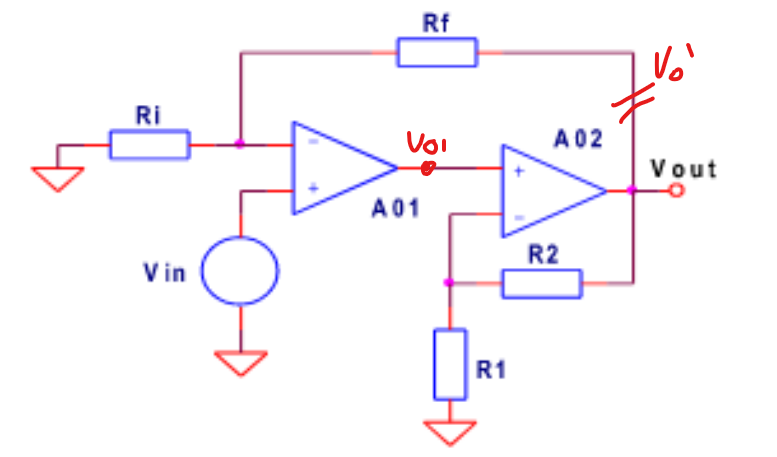
\includegraphics[height=5cm]{Imágenes/vfavfa.png}
    \caption{Amplificador Compuesto VFA-VFA}
\end{figure}

La respuesta de segundo orden del amplificador operacional 1, tiene la siguiente función de transferencia:\\

\begin{center}
    \boxed{Ad(s) = \frac{A_{do}}{(1+\frac{s}{\omega_1}) * (1+\frac{s}{\omega_2})}}\\
\end{center}

\begin{figure}[ht]
    \centering
    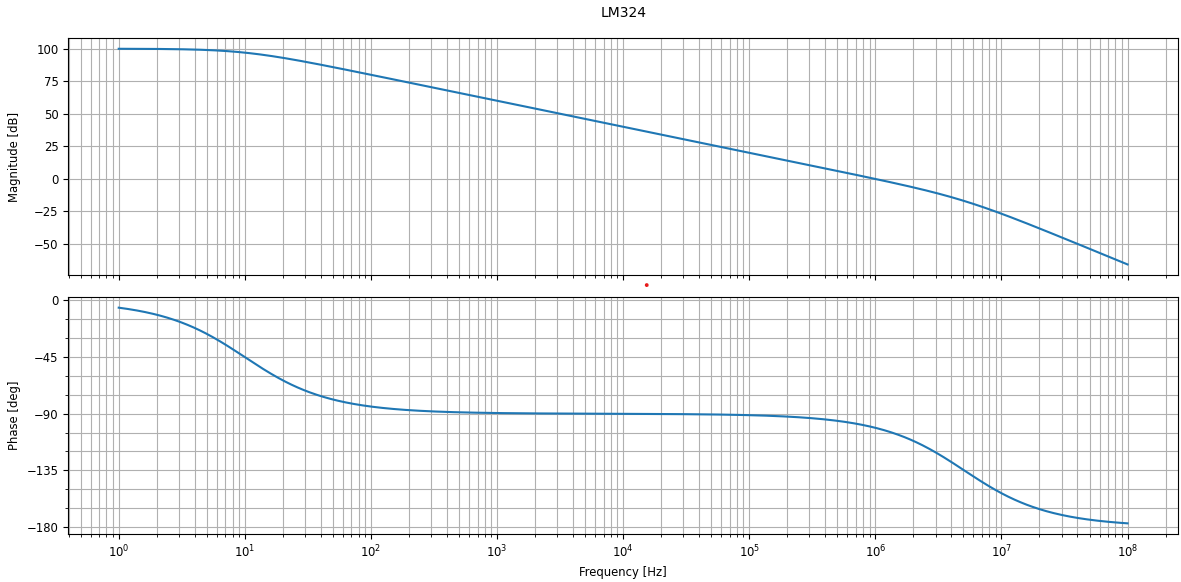
\includegraphics[height=8cm]{Imágenes/lm324.png}
    \caption{Bode de la respuesta del AO}
\end{figure}

\subsubsection{Ganancia de Lazo $T(s)$:}
Se define como:\\

\begin{center}
    \boxed{T(s) = \frac{V_{out}}{V_o'}}\\
\end{center}

$T(s) = \frac{R_i}{R_i + R_f}*-Ad(s)*(1 + \frac{R_2}{R_1})$\\

\begin{center}
    \boxed{T(s) = - \frac{A_{do}}{(1+\frac{s}{\omega_1}) * (1+\frac{s}{\omega_2})} * \frac{R_i}{R_i + R_f}*(1 + \frac{R_2}{R_1})}\\
\end{center}

\newpage
\subsubsection{Ganancia de Lazo Abierto Av(s):}
Para esto, hay que determinar la siguiente expresión:\\

\begin{center}
    \boxed{Av(s) = \frac{V_{out}}{V_{in}}|_{V_o' = 0}}
\end{center}

$Av(s) = Ad(s)*(1+ \frac{R_2}{R_1}) = Ad(s)*k1$

\begin{center}
    \boxed{Av(s) = \frac{A_{do}}{(1+\frac{s}{\omega_1}) * (1+\frac{s}{\omega_2})}*(1+ \frac{R_2}{R_1})}
\end{center}

\subsubsection{Ganancia de Lazo Cerrado Avf(s):}
Se define mediante \textbf{Blackman} como:

\[Avf(s) = \frac{Av(s)}{1-T(s)}\]

Si reemplazamos y simplificamos la expresión (Tomando límite de Ad0 a infinito), se obtiene:

\[Avf(s) = \frac{Ad(s)\cdot (1 + \frac{R_2}{R_1})}{1+Ad(s)\cdot \frac{R_i}{R_i + R_f}\cdot (1 + \frac{R_2}{R_1})}\]

\begin{center}
    \boxed{Avf = \frac{R_i + R_f}{R_i}}
\end{center}

Se pide obtener una ganancia de $Avf = 20 [dB] = 10$, por lo cual la relación entre las resistencias tendrá que ser de:\\

$\frac{R_f}{R_i} = 9 \xrightarrow{} R_f = 90 [k\Omega], R_i = 10 [k\Omega]$\\

Podemos verificar que la ganancia de lazo cerrado casi no depende de $R_1$ y $R_2$, estas serán un parámetro a ajustar para el margen de fase deseado de $M\phi = 65^o$:\\

Por lo que a lazo cerrado será:\\

\begin{center}
    \boxed{Avf(s) = \frac{Av(s)}{1+Av(s)*0.1}}
\end{center}

Para hayar el márgen de fase, y utilizando las herramientas de bode (Simplificando asintóticamente):\\

\[-20 = \frac{20 - (Ado|_{dB} + k1|_{dB})}{log(\omega_g) - log(\omega_1)} \xrightarrow{} \omega_g = 628230*(1.122)^{k_{1}}\]

Si a esto lo colocamos en el margen de fase deseado:\\

$M\phi = 65^o = 180^o - arctg(\frac{628230*(1.122)^{k_{1}}}{\omega_1}) - arctg(\frac{628230*(1.122)^{k_{1}}}{\omega_2})$\\

De aquí despejamos $K_1$:\\

\begin{center}
    \boxed{k_1 = 27.46|_{dB}}
\end{center}

Por lo que en ganancia sería $k_1 = 23.6$ y recordando que $k_1 = 1 +\frac{R_2}{R_1}$, hayamos:\\

\begin{center}
    \boxed{R_1 = 1 [k\Omega]}
\end{center}
\begin{center}
    \boxed{R_2 = 22.6 [k\Omega]}
\end{center}

Ahora podemos verificar lo calculado mediante python, dándonos la siguiente respuesta:\\

\begin{figure}[ht]
    \centering
    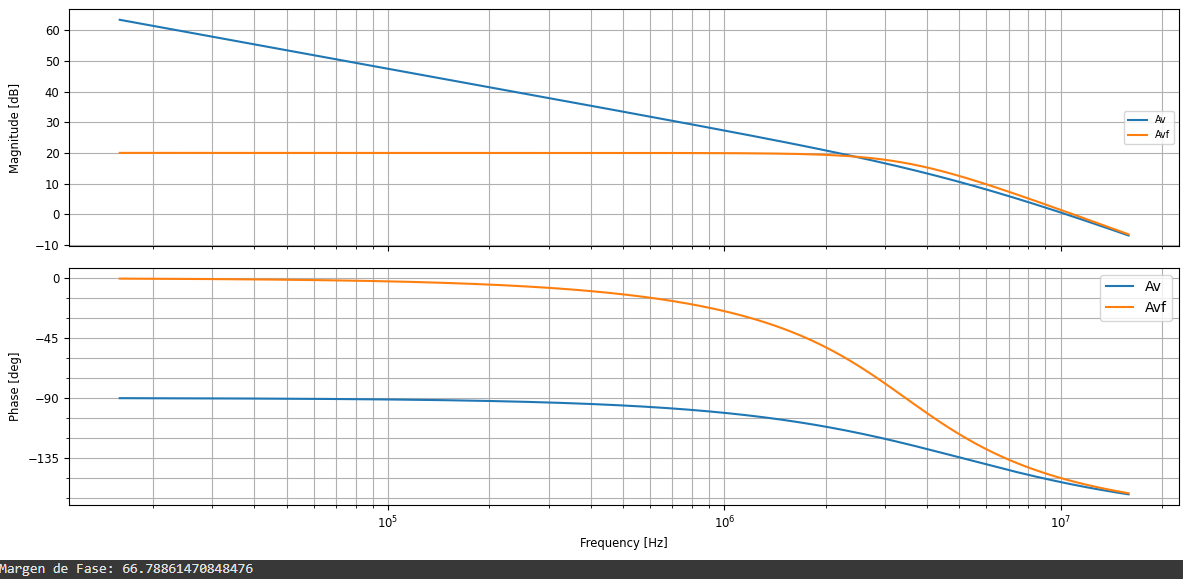
\includegraphics[height=8cm]{Imágenes/VFA_VFA.png}
    \caption{Respuesta en lazo cerrado}
\end{figure}

Ahora, el ancho de banda potencial, lo podemos estimar mediante la constante anteriormente determinada, de modo que $\omega_g = 628230*(1.122)^{k_{1}}$:\\

\begin{center}
    \boxed{f_g = 2.36 [MHz]}
\end{center}

Podemos estimar el margen de fase mediante el sobrepasamiento de la respuesta al impulso:

\begin{figure}[ht]
    \centering
    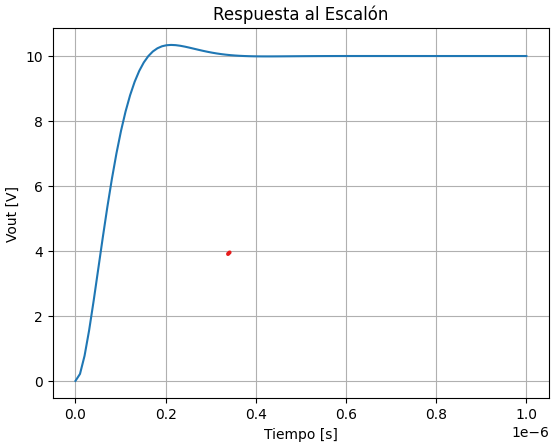
\includegraphics[height=5cm]{Imágenes/VFA_VFA_Escalon.png}
    \caption{Respuesta al escalón}
\end{figure}


El sobrepasamiento $M_p\% = 3.41$, esto nos da un psita $\zeta = 0.73$, estimando el margen de fase:

\begin{center}
    \boxed{M\phi \approx 100*\zeta = 73}
\end{center}

\newpage

\subsubsection{Simulaciones}
\begin{figure}[H]
    \centering
    \begin{minipage}{0.48\textwidth}
        \centering
        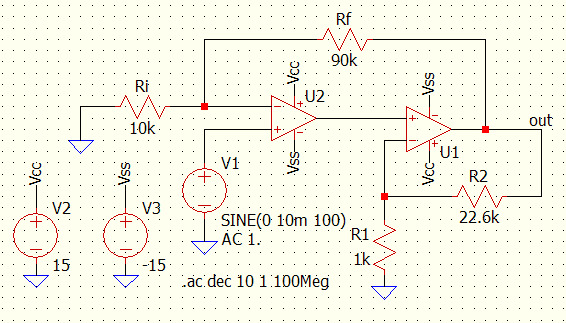
\includegraphics[height=5cm]{Imágenes/vfa vfa diagrama.jpeg}
        \caption{Diagrama de Real VFA-VFA}
        \label{fig:diagrama_vos}
    \end{minipage}
    \hfill
    \begin{minipage}{0.48\textwidth}
        \centering
        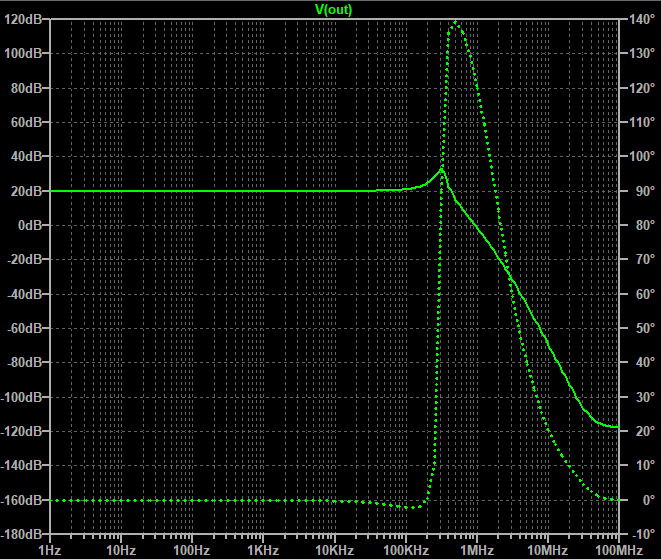
\includegraphics[height=5cm, width=8cm]{Imágenes/vfa vfa bode.jpeg}
        \caption{Simulación Bode VFA-VFA}
        \label{fig:simu_vos}
    \end{minipage}
\end{figure}

La respuesta en frecuencia se obtiene debido a las limitaciones del ancho de banda de los amplificadores reales, las capacitancias parasitarias internas y las interacciones entre los componentes pasivos del circuito. Esto genera un pico de resonancia en una banda de frecuencia específica, causado por la realimentación y las propiedades dinámicas del sistema. Finalmente, la ganancia disminuye a altas frecuencias por la limitación del producto ganancia-ancho de banda (GBW) de los amplificadores.


\newpage
\subsection{VFA-CFA}

    Para desarrollar esta parte, se tomará el mismo comportamiento del VFA del caso anterior y con respecto al CFA, su polo de alta frecuencia posee un efecto despreciable con respecto a la respuesta del amplificador en lazo cerrado, en base a esto, el margen de fase quedará determinado por la siguiente expresión:

    \begin{center}
        $M\phi = 180^o -arctg(\frac{f_g}{f_{1VFA}}) -arctg(\frac{f_g}{f_{2VFA}}) -arctg(\frac{f_g}{f_{CFA}})$
    \end{center}

    Que reemplazando por los datos nos da, considerando que queremos un ancho de banda potencial de $f_g = 2[MHz]$:

    \begin{center}
        $65.5^o = 180^o -arctg(\frac{2[MHz]}{10 [Hz]}) -arctg(\frac{2[MHz]}{5.06 [MHz]}) -arctg(\frac{2[MHz]}{f_{CFA}})$ 
    \end{center}

    Esto implica que la frecuencia de corte a -3 [dB] que deberá poseer el CFA a lazo cerrado será de:

    \begin{center}
        \boxed{f_{CFA} = 39.03 [MHz]}
    \end{center}

    Con esta frecuencia de corte y, conociendo la respuesta de un CFA no inversor a lazo cerrado, se procede a calcular $R_2$ a partir de la siguiente ecuación:

    \begin{center}
        $\omega_{CFA} = \frac{1}{C_T*R_2}$
    \end{center}

    \begin{center}
        $R_2 = \frac{1}{4.8pF .2.\pi*39.03 MHz} = 850 \Omega$
    \end{center}

    \begin{center}
        \boxed{R_2 = 850 \Omega}
    \end{center}

    Ahora necesitamos conocer el valor de $R_1$, esto lo podemos hacer mediante el producto de ganancia por ancho de banda que deberá cumplir:

    \begin{center}
        $A_{vf}.f_g = A_{do}.f_1.A_{vfcfa}$
    \end{center}

    Despejando y conociendo la ganancia ideal de lazo cerrado que deberá poseer el CFA:

    \begin{center}
        \boxed{A_{vfcfa} = 20}
    \end{center}

    Y conociendo además que la ganancia de un amplificador no inversor es de:

    \begin{center}
        $A_{vfcfa} = 1 + \frac{R_2}{R_1}$
    \end{center}

    Por lo que la resistencia faltante será de:

    \begin{center}
        \boxed{R_1 = 44.7 \Omega}
    \end{center}

    Para tener la ganancia de lazo cerrado total especificada de 20 [dB], las resistencias del VFA serán las mismas que en anterior caso.

    Graficando el bode mediante Python para el caso de lazo abierto y lazo cerrado, podemos corroborar que se cumplen las condiciones dadas:

    \begin{figure}[h]
        \centering
        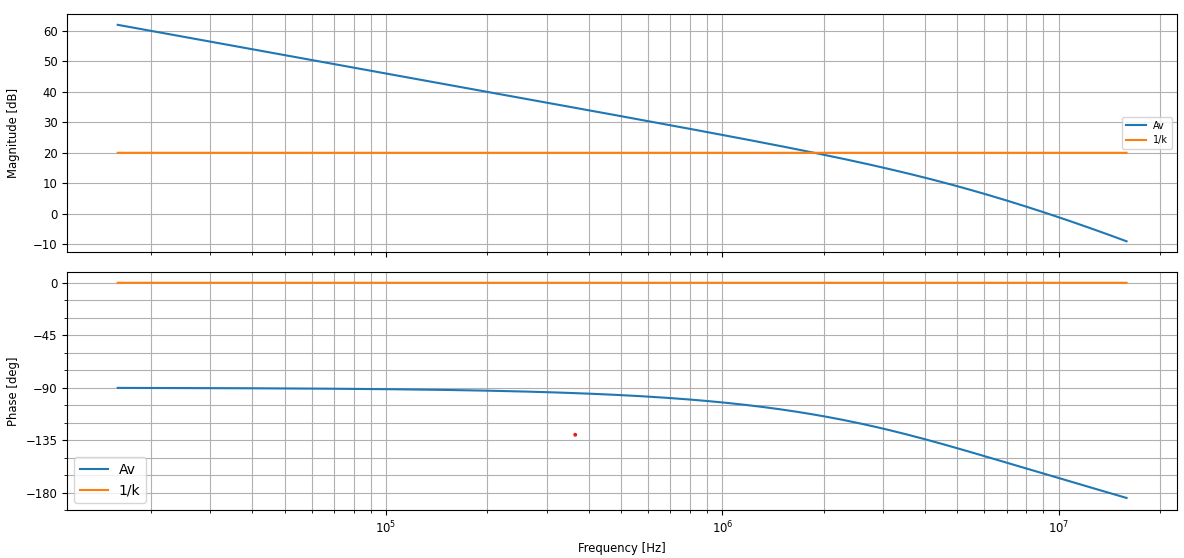
\includegraphics[height=8cm]{Imágenes/VFACFA1.png}
        \caption{Lazo Abierto VFA-CFA}
    \end{figure}
    
    \begin{figure}[h]
        \centering
        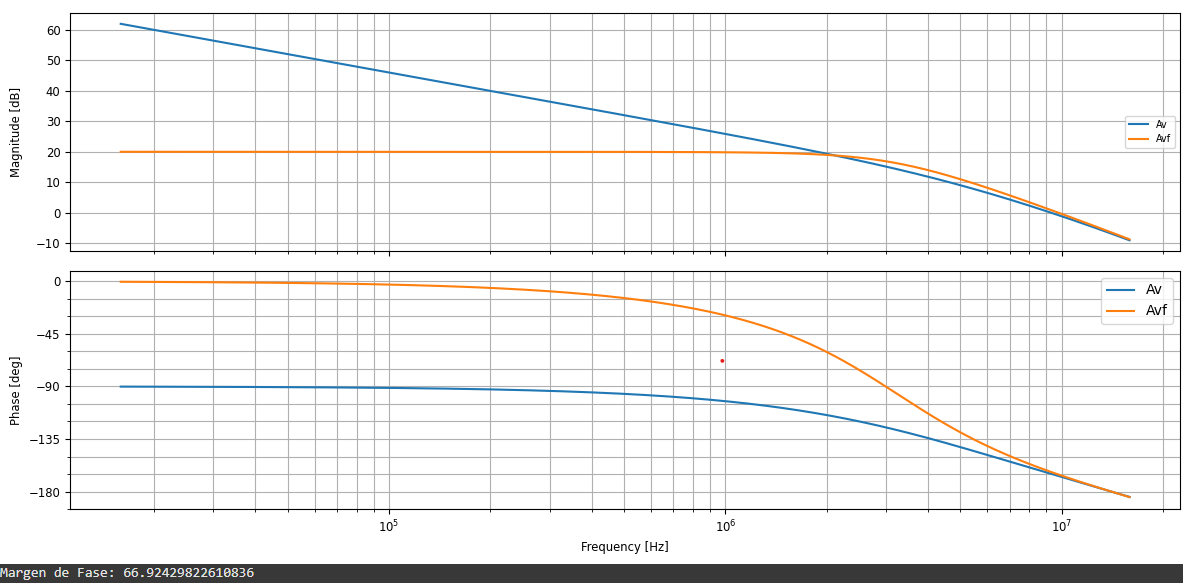
\includegraphics[height=8cm]{Imágenes/VFACFA2.png}
        \caption{Lazo Cerrado VFA-CFA}
    \end{figure}

    \newpage
    \subsubsection{Simulaciones}
\begin{figure}[H]
    \centering
    \begin{minipage}{0.48\textwidth}
        \centering
        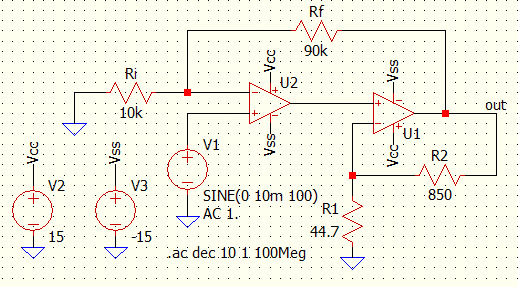
\includegraphics[height=5cm]{Imágenes/vfa cfa diagrama.jpeg}
        \caption{Diagrama de Real VFA-CFA}
        \label{fig:diagrama_vos}
    \end{minipage}
    \hfill
    \begin{minipage}{0.48\textwidth}
        \centering
        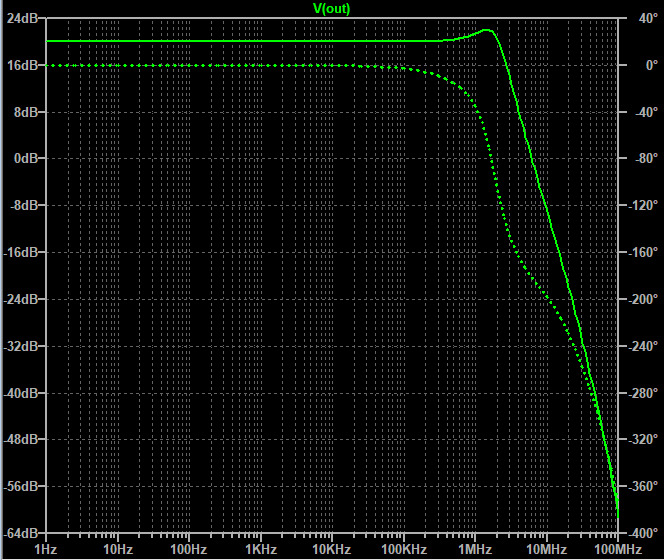
\includegraphics[height=5cm, width=8cm]{Imágenes/vfa cfa bode.jpeg}
        \caption{Simulación Bode VFA-CFA}
        \label{fig:simu_vos}
    \end{minipage}
\end{figure}
La combinación de un VFA con un CFA mejora el desempeño en altas frecuencias gracias al mayor ancho de banda del CFA, reduciendo la caída de ganancia de manera más gradual. A bajas frecuencias, la ganancia es constante y controlada por las resistencias del circuito. Sin embargo, a frecuencias muy altas, las limitaciones internas de ambos amplificadores y las capacitancias parasitarias causan una caída final en la ganancia.

    \subsection{VFA-CFA Compensado}
    
    A la anterior configuración ya dada, se procede a añadir una red de compensación cero-polo, con el propósito de cancelar el polo de alta frecuencia del VFA ubidcado en 5.06 MHz, esta red de compensación estará ubicada a la salida del VFA de manera que cambiará la respuesta a lazo abierto del sistema en su totalidad:

    \begin{figure}[ht]
        \centering
        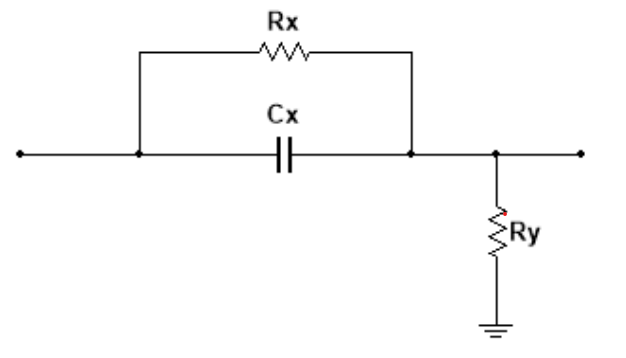
\includegraphics[height=7cm]{Imágenes/red.png}
        \caption{Red de Compensación pasiva RC (cero-polo)}
    \end{figure}

    La función de transferencia de esta red será la siguiente:

    \begin{center}
        $C(s) = \frac{R_y}{R_x + R_y} * \frac{ 1 + s.C_x.R_x}{ 1 + s.C_x.(R_x//R_y)}$
    \end{center}

    En donde los elementos claves serán:

    \begin{center}
        \boxed{C(s) = Comp(0).\frac{ 1 + \frac{s}{\omega_z}}{ 1 + \frac{s}{\omega_p}}}
    \end{center}

    Donde:

    \begin{itemize}
        \item Comp(0) = $\frac{R_y}{R_x + R_y}$ Ganancia Estática.
        \item $\omega_z$ = $\frac{1}{C_x.R_x}$ Cero de la FT.
        \item $\omega_p$ = $\frac{1}{C_x.(R_x//R_y)}$ Polo de la FT.
    \end{itemize}

    Como debemos cancelar el segundo polo del CFA con el cero de la red de compensación:

    \begin{center}
        \boxed{\omega_z = \omega_2 = 2.\pi.5.06[MHz]}
    \end{center}

    Además se solicita que el polo de la red de compensación se debe ubicar una octava mayor al cero, entonces resulta que:

    \begin{center}
        \boxed{\omega_p = \omega_z * 2 = 2.\pi.10.12[MHz]}
    \end{center}

    Una relación que proviene del diseño de esta red es la siguiente y nos permitirá calcular directamente la ganancia estática de la misma:

    \begin{center}
        \boxed{Comp(0) = \frac{\omega_z}{\omega_p} = 0.5}
    \end{center}

    Con todos estos datos procedemos a calcular el valor de cada resistencia que tomará en juego esta red:

    \begin{center}
        $0.5 = \frac{R_y}{R_y + R_x} \xrightarrow{} R_y = R_x$
    \end{center}

    \begin{center}
        \boxed{R_x = R_y = 1 [K\Omega]}
    \end{center}

    Además, el valor del capacitor será de:

    \begin{center}
        $\omega_z = \frac{1}{C_x.R_x}$
    \end{center}

    \begin{center}
        \boxed{C_x = 31 [pF]}
    \end{center}

    Al agregar este compensador, obtendremos la siguiente respuesta a lazo abierto (despreciando el segundo polo del CFA).

    \begin{center}
        $A_v(s)= \frac{Ado}{(1+ \frac{s}{\omega_1}).(1+ \frac{s}{\omega_2})} * comp(0)*\frac{(1+\frac{s}{\omega_z})}{(1+\frac{s}{\omega_p})} * \frac{A_{vfcfa}}{(1+\frac{s}{\omega_{cfa}})}$
    \end{center}

    El cual simplificado quedará de la siguiente forma:

    \begin{center}
        \boxed{\frac{Ado*comp(0)*A_{vfcfa}}{(1+\frac{s}{\omega_1})*(1+\frac{s}{\omega_{cfa}})*(1 + \frac{s}{\omega_p})}}
    \end{center}

    Podemos ver que al agregar esta red de compensación, se atenúa la ganancia en lazo abierto, por lo cual debemos compensarla ajustando la ganancia del CFA de manera que compense el mismo.

    Por lo que si duplicamos la ganancia del CFA tal que:

    \begin{center}
        $A_{vfcfa} = 40 = 1 + \frac{R_2}{R_1}$
    \end{center}

    Con $R_2 = 850\Omega$ siendo este el que no cambiará, entonces:

    \begin{center}
        \boxed{R_1 = 21.8\Omega}
    \end{center}
    
    El margen de fase para este sistema compensado, será el siguiente:

    \begin{center}
        $M\phi = 180 - arctg(\frac{f_g}{f_1}) - arctg(\frac{f_g}{f_p}) - arctg(\frac{f_g}{f_{cfa}})$
    \end{center}

    \begin{center}
        $M\phi = 180 - arctg(\frac{2 [MHz]}{10 [Hz]}) - arctg(\frac{2 [MHz]}{10.12 [MHz]}) - arctg(\frac{2 [MHz]}{39.03 [MHz]})$
    \end{center}

    \begin{center}
        \boxed{M\phi = 75.89^o}
    \end{center}

    Por lo que podemos ver, mejoramos el margen de fase del sistema agregando esta red de compensación.

    A continuación se adjuntan diagramas de bode a lazo cerrado y lazo abierto de este sistema:

    \begin{figure}[h]
        \centering
        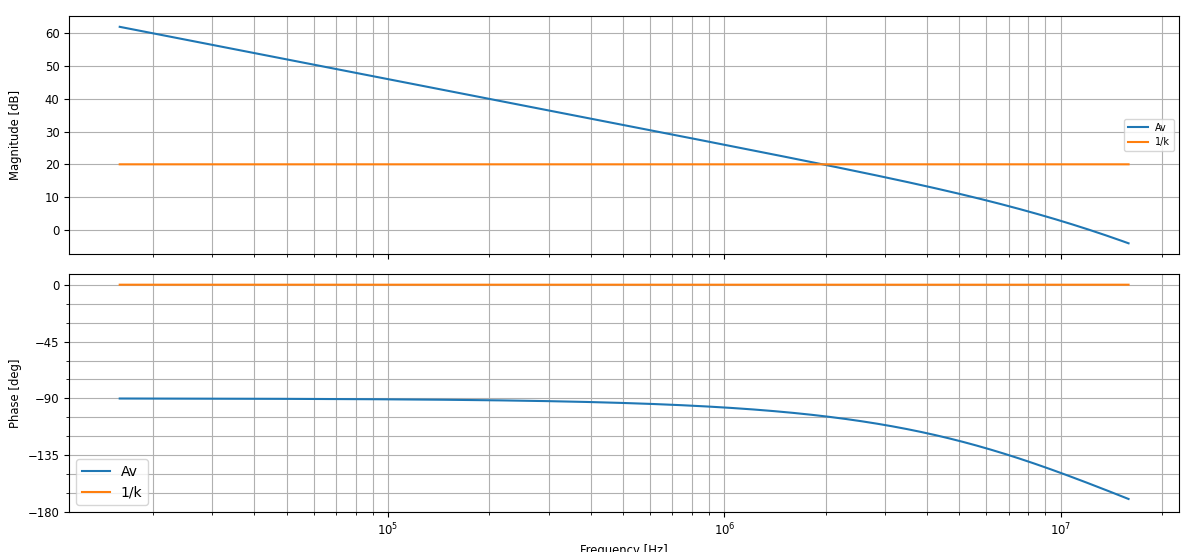
\includegraphics[height=8cm]{Imágenes/VFACFAComp1.png}
        \caption{Lazo Abierto VFA-CFA Compensado}
    \end{figure}
    
    \begin{figure}[h]
        \centering
        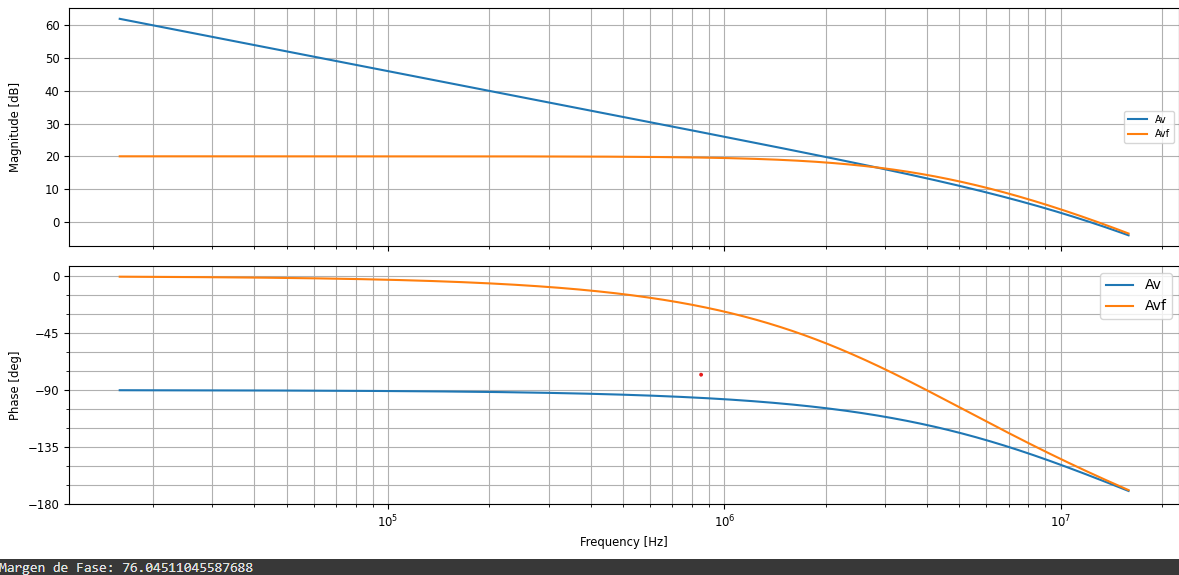
\includegraphics[height=8cm]{Imágenes/VFACFAComp2.png}
        \caption{Lazo Cerrado VFA-CFA Compensado}
    \end{figure}


    \newpage
    \subsubsection{Simulaciones}
    \begin{figure}[H]
    \centering
    \begin{minipage}{0.48\textwidth}
        \centering
        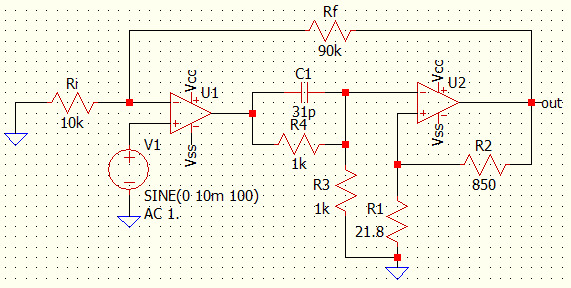
\includegraphics[height=5cm, width=7cm]{Imágenes/WhatsApp Image 2024-12-01 at 07.04.22.jpeg}
        \caption{Diagrama Real VFA-CFA Compensado}
        \label{fig:diagrama_vos}
    \end{minipage}
    \hfill
    \begin{minipage}{0.48\textwidth}
        \centering
        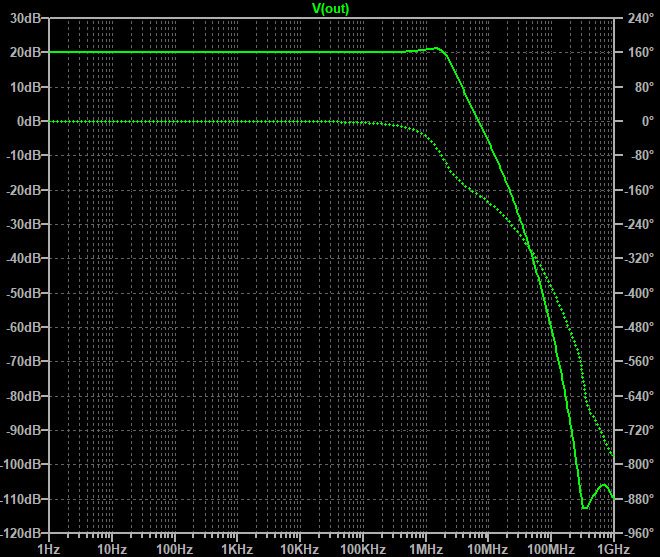
\includegraphics[height=5cm, width=8cm]{Imágenes/WhatsApp Image 2024-12-01 at 07.03.10.jpeg}
        \caption{Simulación Bode VFA-CFA Compensado}
        \label{fig:simu_vos}
    \end{minipage}
\end{figure}
Colocando una compensación polo-cero entre el VFA y el CFA, el circuito mejora su estabilidad y respuesta en frecuencia. El polo ayuda a reducir la ganancia en altas frecuencias, controlando posibles oscilaciones, mientras que el cero incrementa la ganancia en una banda específica para compensar la caída inicial. Esto puede suavizar la transición en la respuesta de ganancia, minimizando resonancias y mejorando el margen de fase, logrando un sistema más estable y con mejor desempeño dinámico.